\documentclass{beamer}

\usepackage{algorithm}
\usepackage{algpseudocode}

\usefonttheme{serif}
\usepackage{dsfont}
\setbeamersize{text margin left=5pt, text margin right=5pt}

\newcommand{\bgk}[1]{\boldsymbol{#1}}

\newcommand{\bzero}{\bgk{0}}
\newcommand{\bone}{\bgk{1}}

\newcommand{\balpha}{\bgk{\alpha}}
\newcommand{\bnu}{\bgk{\nu}}
\newcommand{\bbeta}{\bgk{\beta}}
\newcommand{\bxi}{\bgk{\xi}}
\newcommand{\bgamma}{\bgk{\gamma}} 
\newcommand{\bo}{\bgk{o }}
\newcommand{\bdelta}{\bgk{\delta}}
\newcommand{\bpi}{\bgk{\pi}}
\newcommand{\bepsilon}{\bgk{\epsilon}} 
\newcommand{\bvarepsilon}{\bgk{\varepsilon}} 
\newcommand{\brho}{\bgk{\rho}}
\newcommand{\bvarrho}{\bgk{\varrho}}
\newcommand{\bzeta}{\bgk{\zeta}}
\newcommand{\bsigma}{\bgk{\sigma}}
\newcommand{\boldeta}{\bgk{\eta}}
\newcommand{\btay}{\bgk{\tau}}
\newcommand{\btheta}{\bgk{\theta}}
\newcommand{\bvertheta}{\bgk{\vartheta}}
\newcommand{\bupsilon}{\bgk{\upsilon}}
\newcommand{\biota}{\bgk{\iota}}
\newcommand{\bphi}{\bgk{\phi}}
\newcommand{\bvarphi}{\bgk{\varphi}}
\newcommand{\bkappa}{\bgk{\kappa}}
\newcommand{\bchi}{\bgk{\chi}}
\newcommand{\blambda}{\bgk{\lambda}}
\newcommand{\bpsi}{\bgk{\psi}}
\newcommand{\bmu}{\bgk{\mu}}
\newcommand{\bomega}{\bgk{\omega}}

\newcommand{\bA}{\bgk{A}}
\newcommand{\bDelta}{\bgk{\Delta}}
\newcommand{\bLambda}{\bgk{\Lambda}}
\newcommand{\bSigma}{\bgk{\Sigma}}
\newcommand{\bOmega}{\bgk{\Omega}}
\newcommand{\bPsi}{\bgk{\Psi}}

\newcommand{\bvec}[1]{\mathbf{#1}}

\newcommand{\va}{\bvec{a}}
\newcommand{\vb}{\bvec{b}}
\newcommand{\vc}{\bvec{c}}
\newcommand{\vd}{\bvec{d}}
\newcommand{\ve}{\bvec{e}}
\newcommand{\vf}{\bvec{f}}
\newcommand{\vg}{\bvec{g}}
\newcommand{\vh}{\bvec{h}}
\newcommand{\vi}{\bvec{i}}
\newcommand{\vj}{\bvec{j}}
\newcommand{\vk}{\bvec{k}}
\newcommand{\vl}{\bvec{l}}
\newcommand{\vm}{\bvec{m}}
\newcommand{\vn}{\bvec{n}}
\newcommand{\vo}{\bvec{o}}
\newcommand{\vp}{\bvec{p}}
\newcommand{\vq}{\bvec{q}}
\newcommand{\vr}{\bvec{r}}
\newcommand{\vs}{\bvec{s}}
\newcommand{\vt}{\bvec{t}}
\newcommand{\vu}{\bvec{u}}
\newcommand{\vv}{\bvec{v}}
\newcommand{\vw}{\bvec{w}}
\newcommand{\vx}{\bvec{x}}
\newcommand{\vy}{\bvec{y}}
\newcommand{\vz}{\bvec{z}}

\newcommand{\vA}{\bvec{A}}
\newcommand{\vB}{\bvec{B}}
\newcommand{\vC}{\bvec{C}}
\newcommand{\vD}{\bvec{D}}
\newcommand{\vE}{\bvec{E}}
\newcommand{\vF}{\bvec{F}}
\newcommand{\vG}{\bvec{G}}
\newcommand{\vH}{\bvec{H}}
\newcommand{\vI}{\bvec{I}}
\newcommand{\vJ}{\bvec{J}}
\newcommand{\vK}{\bvec{K}}
\newcommand{\vL}{\bvec{L}}
\newcommand{\vM}{\bvec{M}}
\newcommand{\vN}{\bvec{N}}
\newcommand{\vO}{\bvec{O}}
\newcommand{\vP}{\bvec{P}}
\newcommand{\vQ}{\bvec{Q}}
\newcommand{\vR}{\bvec{R}}
\newcommand{\vS}{\bvec{S}}
\newcommand{\vT}{\bvec{T}}
\newcommand{\vU}{\bvec{U}}
\newcommand{\vV}{\bvec{V}}
\newcommand{\vW}{\bvec{W}}
\newcommand{\vX}{\bvec{X}}
\newcommand{\vY}{\bvec{Y}}
\newcommand{\vZ}{\bvec{Z}}

\usepackage{subcaption}
\newcommand{\bitem}{\item[$\bullet$]}

\usepackage{xcolor}
\usepackage[utf8]{inputenc}
\DeclareFontEncoding{LS1}{}{}
\DeclareFontSubstitution{LS1}{stix}{m}{n}
\DeclareSymbolFont{symbols2}{LS1}{stixfrak} {m} {n}
\DeclareMathSymbol{\operp}{\mathbin}{symbols2}{"A8}
\setbeamertemplate{navigation symbols}{}

\usepackage{lipsum}

\newtheorem{proposition}[theorem]{Proposition}

\newcommand\blfootnote[1]{%
  \begingroup
  \renewcommand\thefootnote{}\footnote{#1}%
  \addtocounter{footnote}{-1}%
  \endgroup
}

\addtobeamertemplate{navigation symbols}{}{%
    \usebeamerfont{footline}%
    \usebeamercolor[fg]{footline}%
    \hspace{1em}%
    \insertframenumber/\inserttotalframenumber
}

\title{
Multi-linear Algebra\\
-- Sketching Tucker Decomposition --\\
Lecture 17
}
%\subtitle{Mathematical framework, existence and exactness}

\author{F. M. Faulstich}
\date{26/03/2024}

\begin{document}

\frame{\titlepage}

\begin{frame}{Recall}

\pause 

\begin{itemize}
    \bitem Tucker decomposition:\\
    \pause
    Let $\vA \in \mathbb{R}^{n_1\times ... \times n_d}$. Then
    $$
    \begin{aligned}
    \vA &=
    \sum_{i_1  = 1}^{r_1} \cdots \sum_{i_d  = 1}^{r_d}
\vC[i_1,...,i_d] \cdot \vu_{1,i_1}\otimes \vu_{2,i_2}\otimes \cdots \otimes \vu_{d,i_1}\\
    &= \vC *_{1} \vU_1 *_{2} \vU_2 ... *_{d} \vU_d
    \end{aligned}
    $$

\begin{figure}
    \centering
    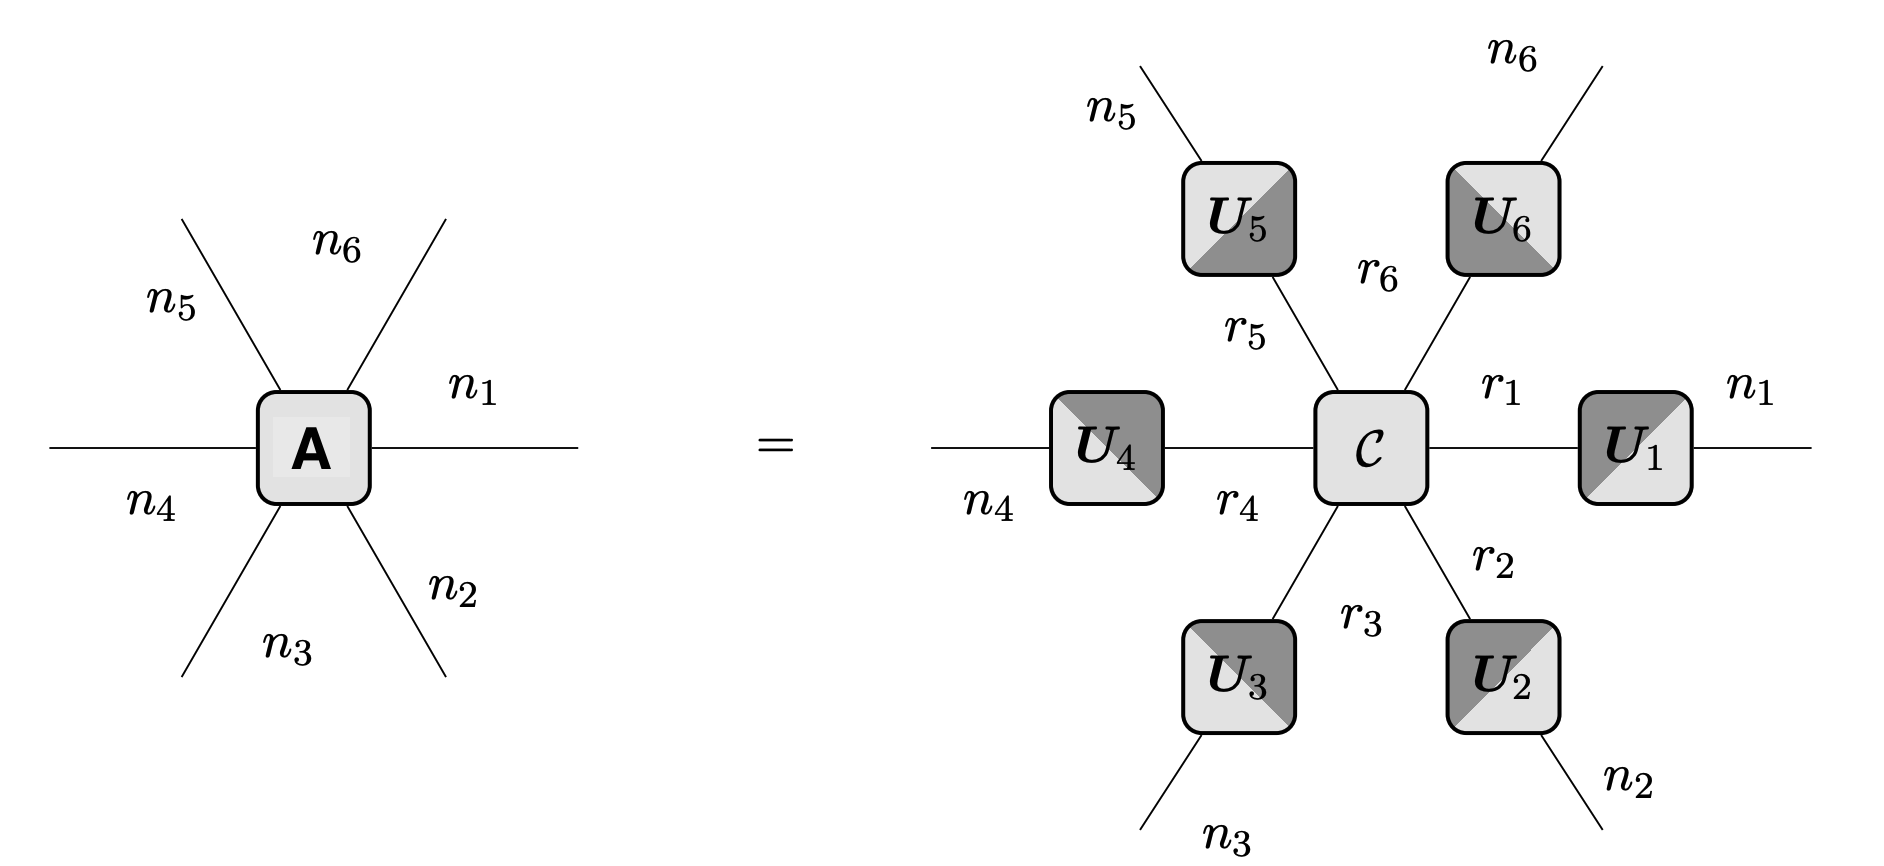
\includegraphics[width=.8\textwidth]{Graphics/TuckerDecomp.png}
\end{figure}
    
\end{itemize}
    
\end{frame}

\begin{frame}{STHOSVD}

{\bf S}equential {\bf T}runcated {\bf H}igher {\bf O}rder SVD (ST-HOSVD)\\
~\\
Algorithm:
    \begin{itemize}
    \item[] Input: Target tensor $\vA\in\mathbb{R}^{n_1\times ... \times n_d}$, target rank $r = (r_1,...,r_d)$
    \item[] Output: Core tensor $\vC$, basis matrices $\vU_k\in \mathbb{R}^{r_k\times n_k}$ for $1\leq k \leq d$
    \item[] Set $\vA_0 = \vA$
    \item[] for $k=1:d$\\
    $\quad $ $\Tilde{\vU}_k, \bSigma_k, \vV_k = {\rm SVD}(\vA_{k-1}^{(k)}, r_k)$\\
    $\quad $ $\vA_k^{(k)} = \bSigma_k \vV_k^\top$\\
    $\quad $ $\vU_k = \Tilde{\vU}_k^\top $
    \item[] $\vC = \vA_d$
\end{itemize}

\end{frame}


\begin{frame}{R-SVD}

\begin{itemize}
    \item[] Input: $\vA \in \mathbb{R}^{m\times n}$, $r\in\mathbb{N}$, $p \in \mathbb{N}$
    \item[] Output: Low-rank approximation of $\vA$: $\hat \vA = \hat \vU \hat \bSigma \hat\vV^\top$
    \item[]  $\bOmega \sim \mathcal{N}(\bzero, \vI) \in \mathbb{R}^{n \times (r+p)}$ 
    \item[] $\vY = \vA \bOmega$
    \item[] $\vQ = {\rm ortho}(\vY)$ [QR-decomp.]
    \item[] $\vB = \vQ^\top \vA$ 
    \item[] $\hat\vU \hat\bSigma \hat\vV^\top = {\rm SVD} (\vB, r)$
    \end{itemize}
\end{frame}

\begin{frame}{Application of R-SVD in STHOSVD}

\begin{center}
Let's apply R-SVD instead of regular SVD!\\~\\
R. Minster, A. K. Saibaba, M. E. Kilmer: Randomized algorithms for
low-rank tensor decompositions in the Tucker format. SIAM Journal on
Mathematics of Data Science. 2(1), 189-215 (2020)
\end{center}

    
\end{frame}

\begin{frame}{R-STHOSVD}
\begin{itemize}
    \item[] Input: Target tensor $\vA$, target rank $(r_1,...,r_d)$, $p\in\mathbb{N}$
    \item[] Output: Core tensor $\vC$, basis matrices $\vU_k\in \mathbb{R}^{r_k\times n_k}$ for $1\leq k \leq d$
    \item[] Set $\vA_0 = \vA$
    \item[] for $k=1:d$\\
    $\quad $ $\Tilde{\vU}_k,~ \bSigma_k,~ \vV_k = \text{ R-SVD}(\vA_{k-1}^{(k)},  r_k, p)$\\
    $\quad $ $\vA_k^{(k)} = \bSigma_k \vV_k^\top$\\
    $\quad $ $\vU_k = \Tilde{\vU}_k^\top $
    \item[] $\vC = \vA_d$
\end{itemize}

\pause
\begin{itemize}
	\bitem What if both matrix dimensions are large?\\
    \pause
	$\rightarrow$ Two-sided sketching\footnote{Tropp, et al. SIAM Journal on Matrix
Analysis Applications. 2017}!
\end{itemize}


\end{frame}


\begin{frame}{Low-rank approximation -- two-sided sketch}

\begin{itemize}
\bitem Choose sketching parameters $r\leq k \leq \min(l,n)$, $0 < l \leq m$
\end{itemize}
Algorithm:
\begin{itemize}
    \item[] Input: $\vA \in \mathbb{R}^{m\times n}$, $k,l\in\mathbb{N}$
    \item[] Output: Rank $r$ approximation of $\vA$: $\hat \vA =  \vQ \vX $
    \item[]  $ \bOmega = \text{ortho}(\tilde\bOmega)\leftarrow \tilde\bOmega \sim \mathcal{N}(\bzero, \vI) \in \mathbb{R}^{n \times k}$
    \item[]  $\bPsi^\top = \text{ortho}(\tilde\bPsi^\top) \leftarrow \tilde\bPsi \sim \mathcal{N}(\bzero, \vI) \in \mathbb{R}^{l \times m}$ 
    \item[] $\vY = \vA \bOmega$
    \item[] $\vW = \bPsi \vA$
    \item[] $\vQ = {\rm ortho}(\vY)$ [QR-decomp.]
    \item[] $\vX = (\bPsi \vQ)^+\vW$
    \end{itemize}

\end{frame}


\begin{frame}{sketched-STHOSVD}

Idea: Use two-sided skeiched low-rank approximation in R-THOSVD\\
~\\
Algorithm:
\begin{itemize}
    \item[] Input: Target tensor $\vA$, target rank $(r_1,...,r_d)$, $(l_1,...,l_d)$
    \item[] Output: Core tensor $\vC$, basis matrices $\vU_k\in \mathbb{R}^{r_k\times n_k}$ for $1\leq k \leq d$
    \item[] Set $\vA_0 = \vA$
    \item[] for $k=1:d$\\
    $\quad $  $\vQ_k, \vX_k = \text{ 2s-r-SVD}(\vA_{k-1}^{(k)},  r_k, l_k)$\\
    $\quad $ Set $\vA_k^{(k)} = \vX_k$\\
    $\quad $ $\vU_k = \vQ_k^\top $
    \item[] $\vC = \vA_d$
\end{itemize}


\end{frame}


\begin{frame}{Sketching with subspace power iteration}

\begin{itemize}
\bitem Spectrum of materialization decays slowly sketching is not great
\bitem Power iteration technique to enhance the sketching algorithm:\\
$\rightarrow$ replace $\vA$ by $(\vA\vA^\top)^q \vA$ for some $q\in\mathbb{N}$
$$
(\vA\vA^\top)^q \vA = \vU \bSigma^{2q+1}  \vV^\top
$$
$\rightarrow$ Left- and right singular vectors remain the same!\\
$\rightarrow$ Faster decay rate of singular values\\ 
$\rightarrow$ Rounding errors may accumulate\\
$\quad$ Remedy: Orthonormalizing the columns of the sample matrix \\
$\qquad\qquad\quad~$ between each application of $\vA$ and $\vA^{\top}$
\end{itemize}


\end{frame}

\begin{frame}{Sketching algorithm with subspace power iteration}

\begin{itemize}
\bitem Choose sketching parameters $r\leq k \leq \min(l,n)$, $0< l \leq m$ 
\end{itemize}
~\\
Algorithm:
\begin{footnotesize}
\begin{itemize}
    \item[] Input: $\vA \in \mathbb{R}^{m\times n}$, $k,l,q\in\mathbb{N}$\vspace{-1.5mm}
    \item[] Output: Rank $r$ approximation of $\vA$: $\hat \vA =  \vQ \vX $\vspace{-1.5mm}
    \item[]  $ \bOmega = \text{ortho}(\tilde\bOmega)\leftarrow \tilde\bOmega \sim \mathcal{N}(\bzero, \vI) \in \mathbb{R}^{n \times k}$\vspace{-1.5mm}
    \item[]  $\bPsi^\top = \text{ortho}(\tilde\bPsi^\top) \leftarrow \tilde\bPsi \sim \mathcal{N}(\bzero, \vI) \in \mathbb{R}^{l \times m}$ \vspace{-1.5mm}
    \item[] $\vY = \vA \bOmega$\vspace{-1.5mm}
    \item[] $\vW = \bPsi \vA$\vspace{-1.5mm}
    \item[] $\vQ_0 = {\rm ortho}(\vY)$ [QR-decomp.]\vspace{-1.5mm}
    \item[] for $j=1:q$\vspace{-1.5mm}
    \item[] $\quad \hat \vY_j = \vA^\top \vQ_{j-1}$\vspace{-1.5mm}
    \item[] $\quad \hat\vQ_j = \text{ortho}(\hat \vY_j)$\vspace{-1.5mm}
    \item[] $\quad \vY_j = \vA\hat \vQ_{j}$\vspace{-1.5mm}
    \item[] $\quad \vQ_j = \text{ortho}( \vY_j)$\vspace{-1.5mm}
    \item[] $\vQ = \vQ_q $\vspace{-1.5mm}
    \item[] $\vX = (\bPsi \vQ)^+\vW$
    \end{itemize}\vspace{-1.5mm}
\end{footnotesize}

\end{frame}


\begin{frame}{sub-sketch-STHOSVD}

Use the sketching algorithm with subspace power iteration in STHOSVD\\
~\\
Algorithm:

\begin{itemize}
    \item[] Input: Target tensor $\vA$, target rank $(r_1,...,r_d)$, $(l_1,...,l_d)$, $q\in\mathbb{N}$
    \item[] Output: Core tensor $\vC$, basis matrices $\vU_k\in \mathbb{R}^{r_k\times n_k}$ for $1\leq k \leq d$
    \item[] Set $\vA_0 = \vA$
    \item[] for $k=1:d$\\
    $\quad $  $\vQ_k, \vX_k = \text{ sub-sketch-SVD}(\vA_{k-1}^{(k)},  r_k, l_k, q)$\\
    $\quad $ Set $\vA_k^{(k)} = \vX_k$\\
    $\quad $ $\vU_k = \vQ_k^\top $
    \item[] $\vC = \vA_d$
\end{itemize}

\end{frame}

\begin{frame}{Comparison}

Experiment 1:\\
~\\
Hilbert tensor $\vA\in\mathbb{R}^{n_1\times ... \times n_d}$:
$$
\vA [i_1,...,i_d]
=
\frac{1}{i_1+...+i_d},
\qquad 
1\leq i_j \leq n_j,~1\leq j \leq d
$$

Tensor parameters:
\begin{itemize}
\bitem $d = 5$  \vspace{-1.5mm}
\bitem $n_j = 25$, $j = 1, 2, . . . , d$ \vspace{-1.5mm}
\bitem Target rank is $(r, r, r, r, r)$, where $r \in [\![1, 25]\!]$
\end{itemize}

Computational parameters:
\begin{itemize}
\bitem Oversampling $p = 5$  \vspace{-1.5mm}
\bitem $l_i = r_i+2$, $i= 1, 2, . . . , d$ \vspace{-1.5mm}
\bitem Power parameter $q=1$
\end{itemize}
\end{frame}

\begin{frame}{}

\begin{figure}
    \centering
    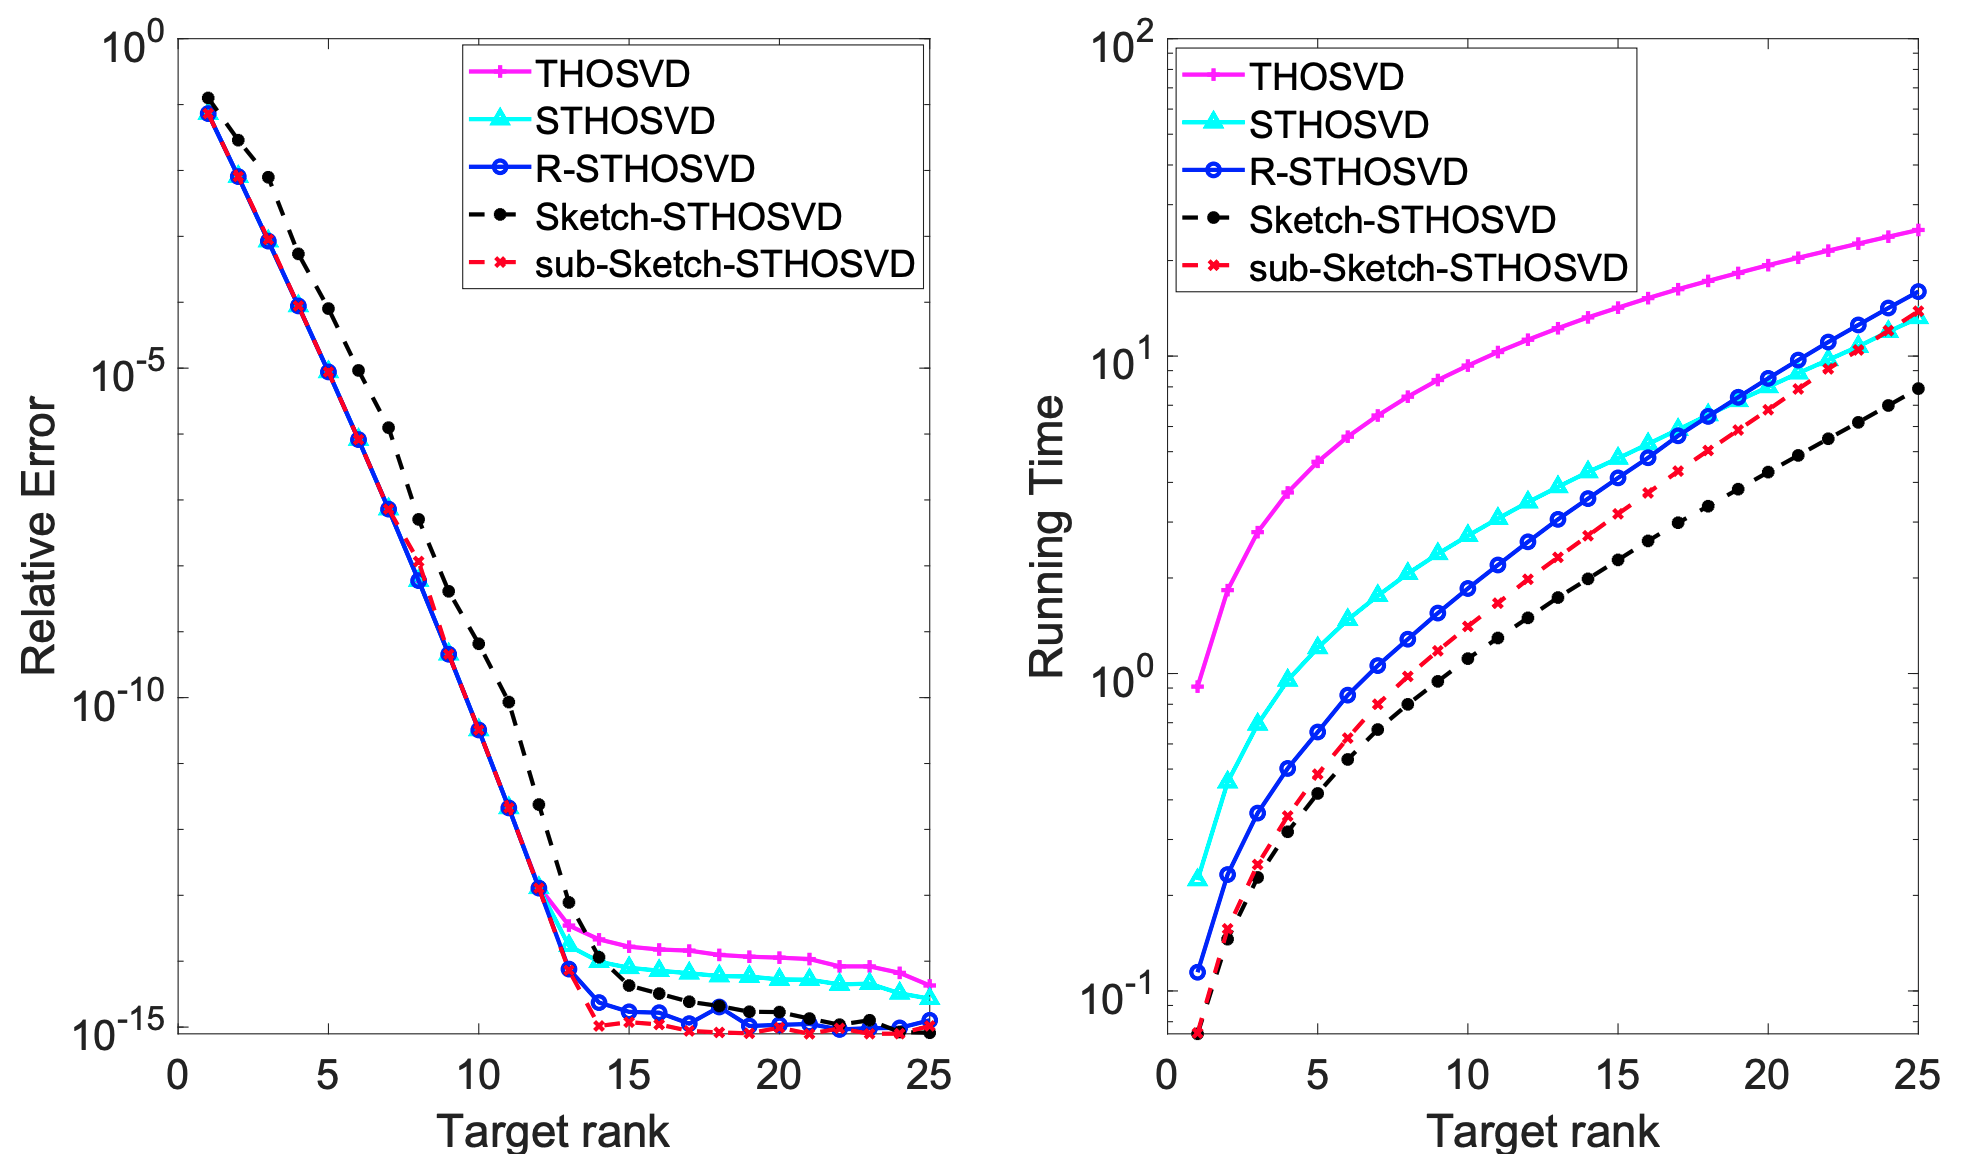
\includegraphics[width =.8\textwidth]{Graphics/HilbertTensor.png}
\end{figure}
\end{frame}

\begin{frame}{}
CPU time (in second) on the Hilbert tensor
with a size of $500 \times 500 \times 500$ as the target rank increases:
\begin{figure}
    \centering
    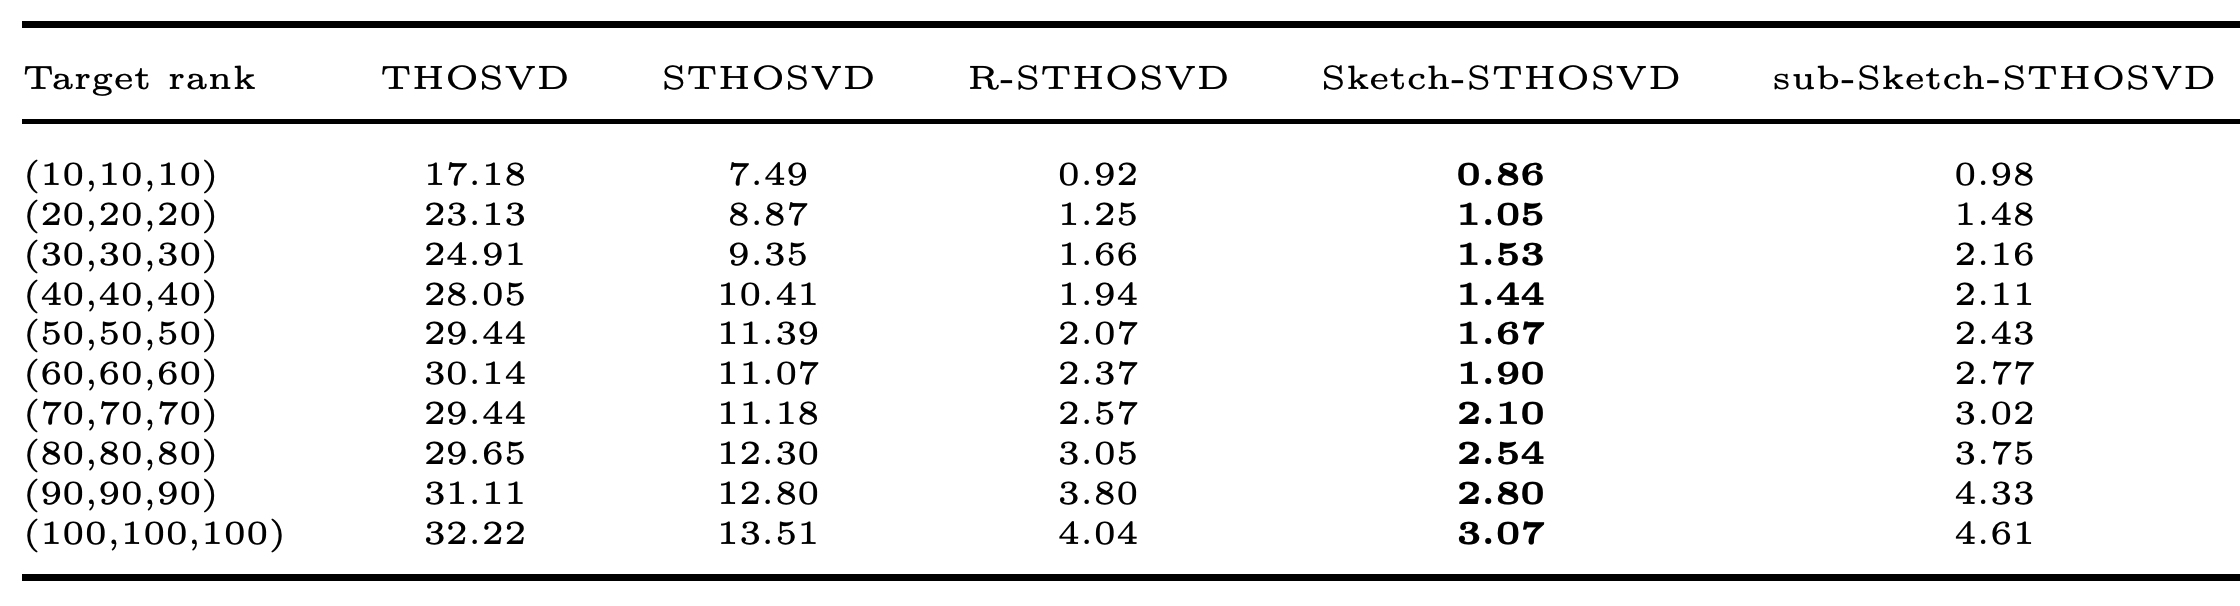
\includegraphics[width =\textwidth]{Graphics/HilbertTab1.png}
\end{figure}

Relative error on the Hilbert tensor with a
size of $500 \times 500 \times 500$ as the target rank increases:
\begin{figure}
    \centering
    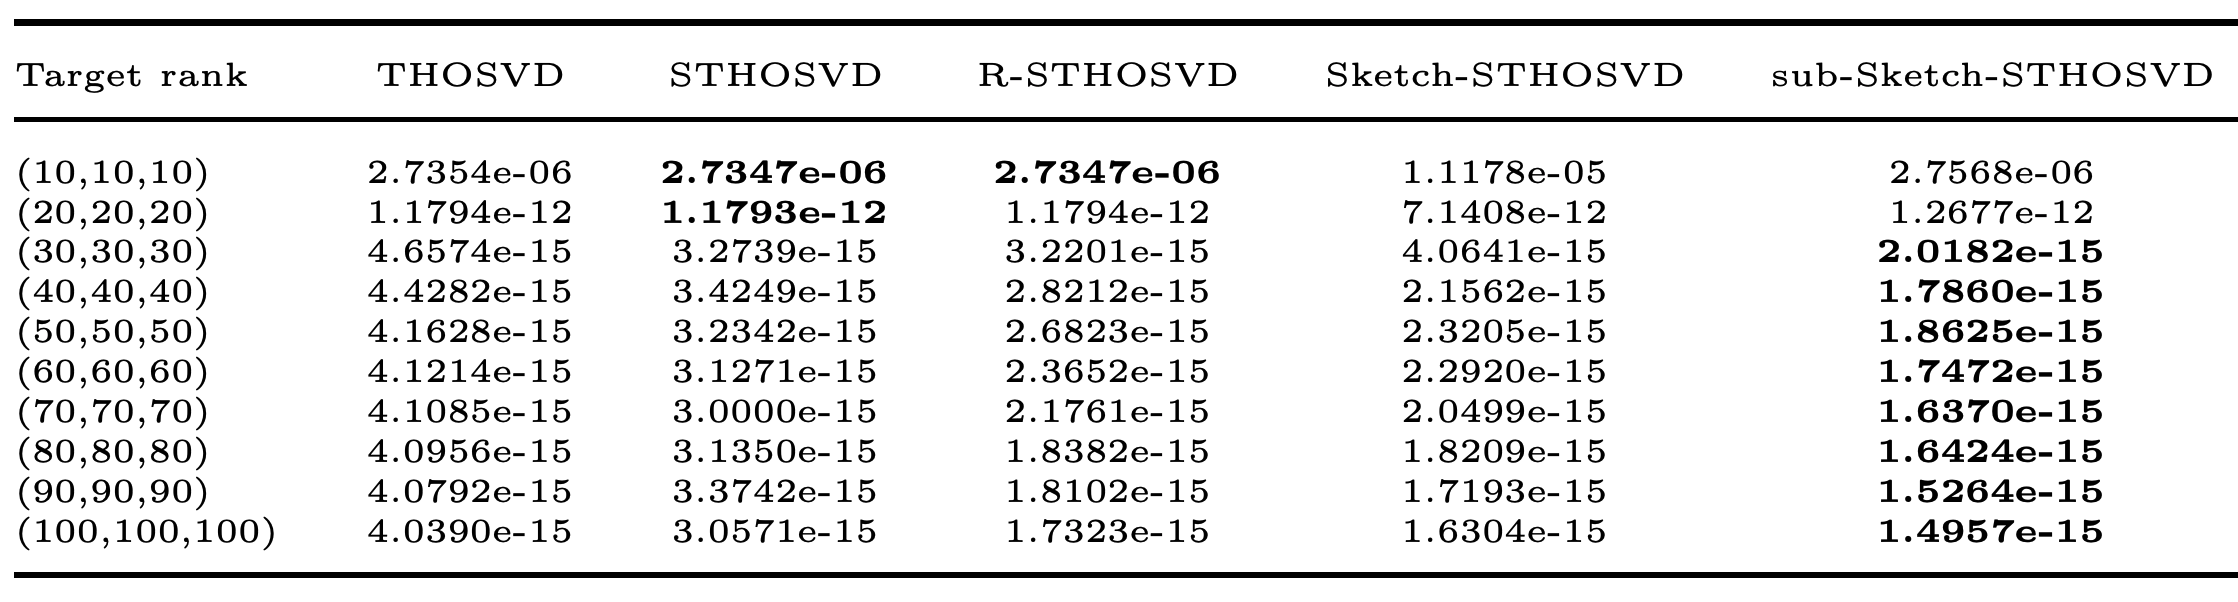
\includegraphics[width =\textwidth]{Graphics/HilbertTab2.png}
\end{figure}
    
\end{frame}

\begin{frame}{Comparison}

Experiment 2:\\
~\\
Sparse tensor $\vA\in\mathbb{R}^{200\times  200 \times 200}$:
$$
\vA 
=
\sum_{i=1}^{10}
\frac{\gamma}{i^2} \vx_i \otimes \vy_i \otimes \vz_i 
+
\sum_{i=11}^{200}
\frac{1}{i^2} \vx_i \otimes \vy_i \otimes \vz_i,
$$
where $ \vx_i ,\vy_i , \vz_i \in \mathbb{R}^{200}$ are sparse vectors with $5\%$ nonzeros each \\
(generated using the \texttt{sprand} command in MATLAB )

Tensor parameters:
\begin{itemize}
\bitem $\gamma = 2, 10, 200$ \vspace{-1.5mm}
\bitem $n_j = 25$, $j = 1, 2, . . . , d$ \vspace{-1.5mm}
\bitem Target rank is $(r, r, r)$, where $r \in [\![20, 100]\!]$
\end{itemize}

Computational parameters:
\begin{itemize}
\bitem Oversampling $p = 5$  \vspace{-1.5mm}
\bitem $l_i = r_i+2$, $i= 1, 2, . . . , d$ \vspace{-1.5mm}
\bitem Power parameter $q=1$
\end{itemize}
\end{frame}

\begin{frame}{}

\begin{figure}
    \centering
    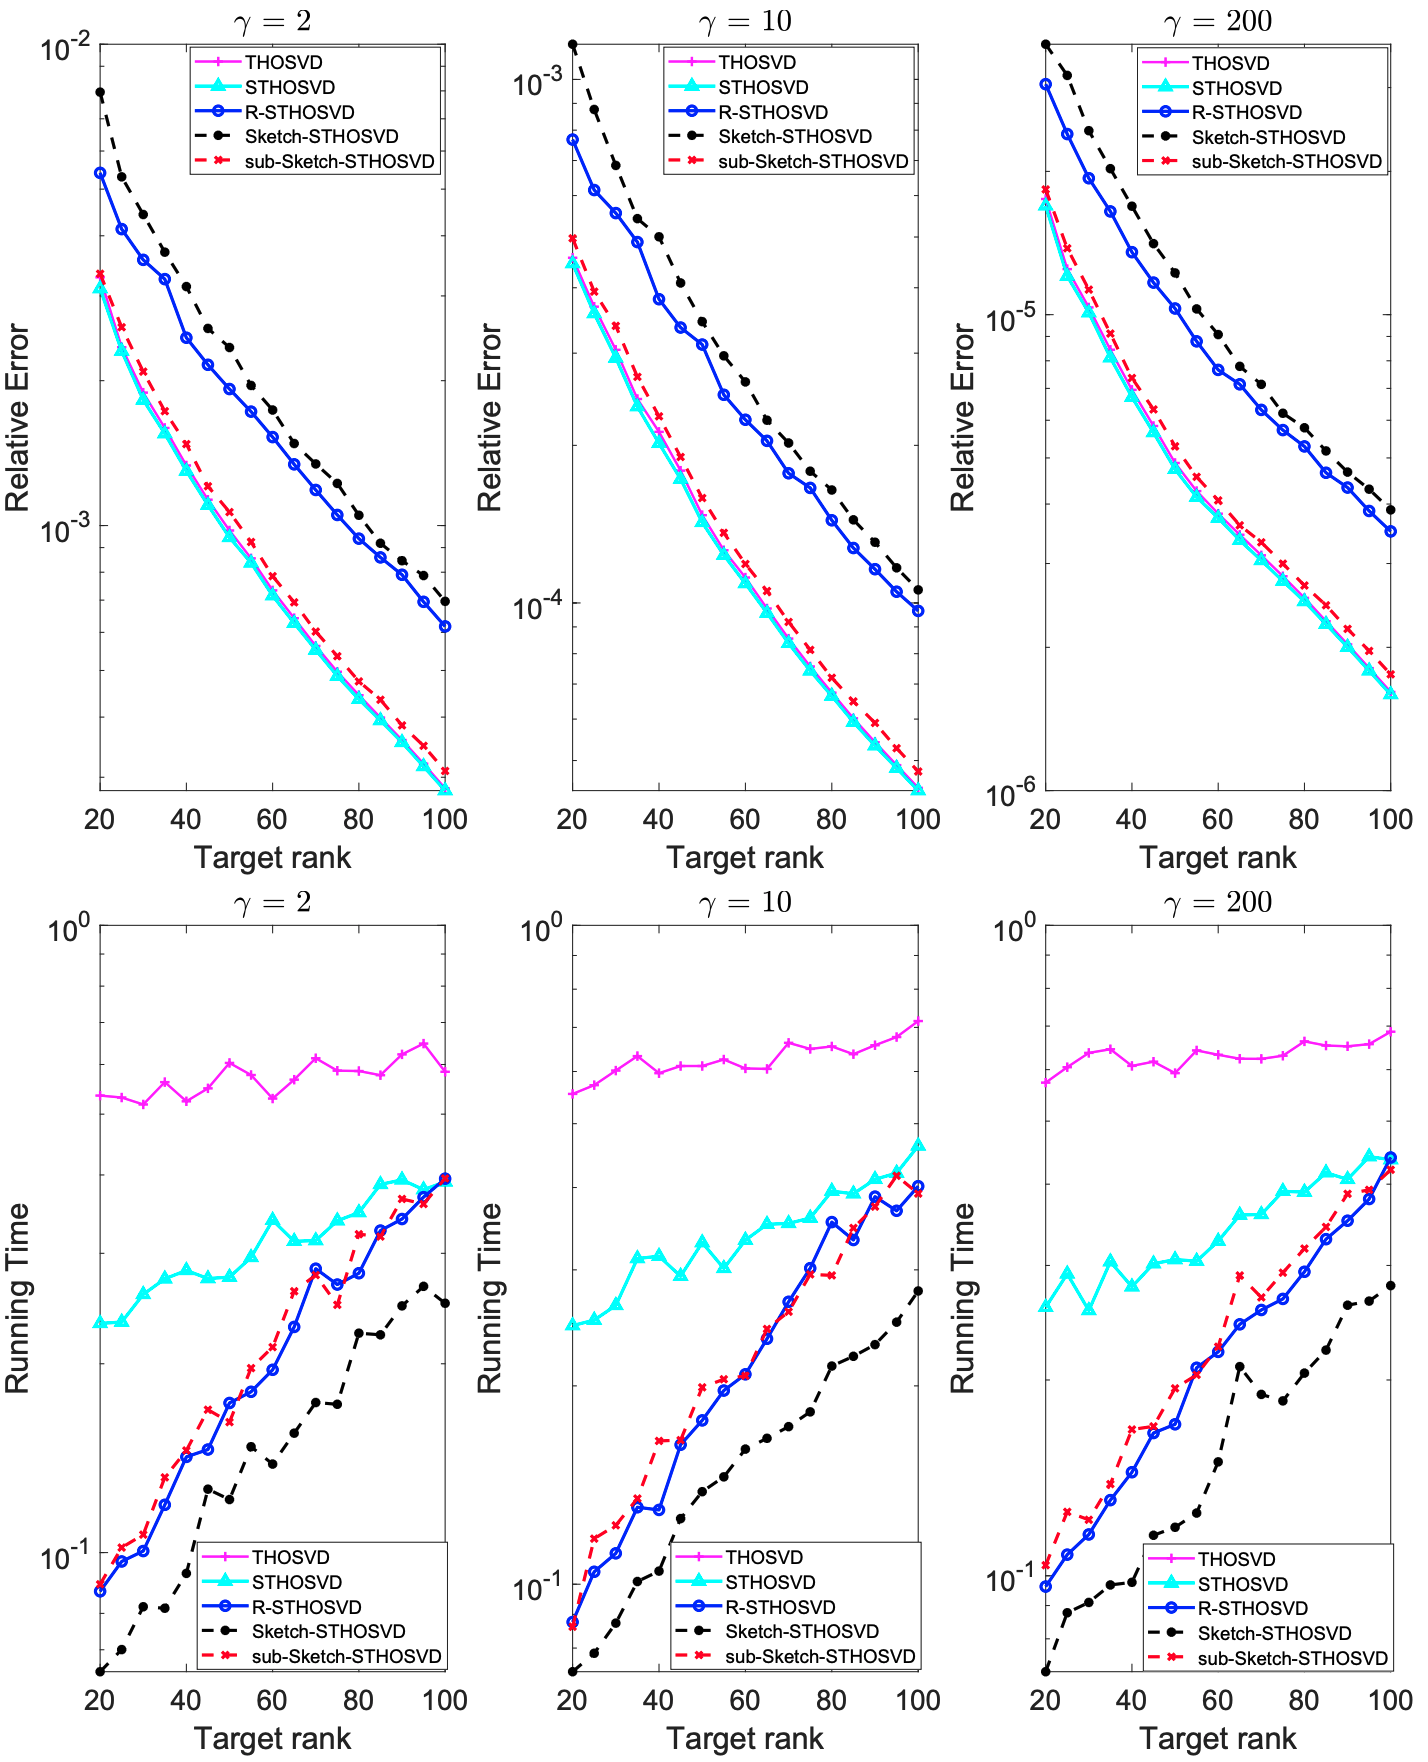
\includegraphics[width = 0.6 \textwidth]{Graphics/SparseFig.png}
\end{figure}
    
\end{frame}


\end{document}




